\documentclass[11pt]{article}
\usepackage[margin=1in]{geometry}
\usepackage[T1]{fontenc}
\usepackage{lmodern,microtype,amsmath,amssymb,amsthm,booktabs,graphicx,xcolor,url}
\usepackage[colorlinks=true,linkcolor=blue!45!black,citecolor=blue!45!black,urlcolor=blue!45!black]{hyperref}
\usepackage{natbib}
\usepackage{enumitem}
\setlist{nosep}
\setlength{\emergencystretch}{2em}
\newtheorem{proposition}{Proposition}
\newtheorem{corollary}{Corollary}
\newcommand{\E}{\mathbb E}
\newcommand{\Pp}{\mathbb P}
\newcommand{\ind}{\mathbf 1}
\newcommand{\R}{\mathbb R}
\title{TAILSENTRY: Structure-Certified Conditional Union Sampling for Rare Losses\\[5pt]\large A Reproducible Study and a Failed Efficiency Hypothesis}
\author{TAILSENTRY computational research artifact\\\small Prepared with Codex; unsubmitted research report}
\date{1 November 2026}
\begin{document}
\maketitle
\begin{abstract}
Rare-event importance sampling can be unbiased and have full support while producing misleading ordinary confidence intervals after missing a catastrophic mode. We implement and audit a specialized alternative: enclose supported maximum-of-quadratic losses in a proved union of halfspaces, sample exact Gaussian or Student conditional components, and integrate one latent Gaussian coordinate using every failure interval. The resulting probability contribution is bounded by the union probability sum, rather than an inverse defensive-mixture fraction. Its unbiasedness and variance dominance over the corresponding raw union sampler follow from established mixture importance sampling and conditional expectation. We do not establish a new general estimator. Across 17,280 complete algorithm runs with independent within-condition replications, eight known-truth problems and 15 methods/variants, the selected fixed-projection estimator failed its prespecified primary comparison: its mean-squared-error times elapsed-time ratio against conditional scrambled Sobol was 38.79 (95\% bootstrap interval 26.48--57.32). A separate randomized-order timing study corroborated the failure. Conditioning improved the raw union sampler, but simpler conditional quasi-Monte Carlo was often stronger. A 512-run omitted-mode counterexample had 0.59\% normal-interval coverage despite approximately 18,000 observed effective tail contributions per run; bounded intervals remained conservative. A separate chronological public-FX check showed a 21.8\% change in 99\% Expected Shortfall between training-fitted distribution families. The contribution is an inspectable implementation, exact conditional-cover derivation, adversarial numerical checks and reproducible positive and negative evidence. Algorithmic originality and a general state-of-the-art breakthrough remain unachieved.
\end{abstract}

\section{Question, scope and outcome}
The scientific question is whether a failure-aware sampler can reduce extreme-loss error at fixed total cost while providing uncertainty that remains meaningful when an entire mechanism is missed. The initial hypothesis favored adaptive mixtures. Prior-art inspection changed the direction: mixture adaptation, defensive exploration, optimized mixture weights and failure-informed subspaces already have substantial precedents \citep{he2014,uribe2021,tong2023,helal2025}. Exact union-event sampling is a particularly strong comparator \citep{owen2019aloe}. It would be misleading to report an improvement over crude Monte Carlo while omitting that structure-aware baseline.

The final implementation focuses on an explicit, limited family of losses. It combines a verifiable structural cover with conditional integration. This trades generic black-box access for mathematical information about the loss function. Our central result is negative: the selected composition did not outperform the strongest applicable simple comparator on the prespecified primary workload. This result does not invalidate conditional variance reduction. It rejects the broader computational efficiency hypothesis for the tested implementation and budget.

Three levels of achievement are kept distinct. The implementation has mathematical and numerical checks. Replicated improvement is observed relative to some comparators and fails relative to others. Originality as a new estimator has not been established. The report and software are not externally peer reviewed, published, regulator-approved or independently adopted.

\section{Related methods and the remaining bottleneck}
Subset simulation expresses a rare probability as a product of less-rare conditional probabilities, with Markov-chain dependence and finite-sample bias requiring care \citep{au2001,openturns}. Cross-entropy methods fit proposals toward progressively rarer sets; failure-informed dimension reduction and large-deviation initialization improve their high-dimensional behavior \citep{uribe2021,tong2023}. SAIS combines subset levels with adaptive multiple importance sampling \citep{helal2025}. A later flow-mixture method, FAMIS, adds defensive exploration and repulsive proposal learning \citep{famis2026}. Latent normalizing-flow exploration provides another route \citep{kruse2025}. We did not reproduce FAMIS or claim dominance over it.

ALOE samples one known union component conditionally and corrects overlaps \citep{owen2019aloe}; defensive adaptive ALOE already addresses selected components and residual exploration \citep{elvira2021}. Conditional simulation for elliptical halfspace unions also predates this project \citep{ahn2018}. Our Gaussian-coordinate marginalization differs from radial integration, but the conditional-expectation principle and broad geometry-assisted direction are established. Bounded-variable confidence procedures are also established \citep{maurer2009,dietrich2026,jain2025}. Recent geometric improvements beyond mean tilting further restrict novelty claims \citep{li2026}.

The practical bottleneck is the distinction between sampled-weight diagnostics and coverage of the target event. A proposal may have positive density everywhere and still encounter a missing mode too rarely for a normal interval to represent actual uncertainty. Sample-size requirements under proposal mismatch can be severe \citep{chatterjee2018}. More elaborate learned proposals cannot provide a generic finite-budget certificate that an arbitrary undiscovered region is negligible.

\section{Supported stochastic model}
Let
\begin{equation}
 X=G/\sqrt{S/\nu},\qquad G\sim N(0,I_d),\quad S\sim\chi^2_\nu,
 \label{eq:student}
\end{equation}
with independent components. The Gaussian case sets the scale identically to one. The Student matrix is a \emph{scale} matrix; its covariance is $\nu I_d/(\nu-2)$ when $\nu>2 $. Correlation and factor loadings can be absorbed into the coefficients below.

The supported loss is
\begin{equation}
 L(x)=\max_{1\le j\le J}\{c_j+a_j^\top x+x^\top B_jx\},\qquad B_j=B_j^\top.
 \label{eq:loss}
\end{equation}
This includes affine stress branches, compact quadratic failure regions, and delta-gamma approximations to short-convexity portfolio losses. Such approximations are prescribed mathematical workloads, not calibrated option-pricing engines. They omit jumps, dynamic hedging, liquidity feedback, transaction costs and path-dependent execution.

For fixed threshold $ t $, the target is $ p_t=\Pp(L(X)>t)$. We also investigate $ q_\alpha=\inf\{q:\Pp(L\le q)\ge\alpha\}$ and
\begin{equation}
 \operatorname{ES}_\alpha=q_\alpha+\frac{\E[(L-q_\alpha)_+]}{1-\alpha}
 \label{eq:es}
\end{equation}
for continuous integrable losses. An unbiased estimator of $ p_t $ does not make quantile inversion or the plug-in expression in\eqref{eq:es} unbiased.

\section{A proved cover and an established union proposal}
For each quadratic branch, write $ B_j=B_j^+-B_j^-$ using its positive and negative eigenspaces. Discarding the nonnegative form $ x^\top B_j^-x $ gives
\begin{equation}
 c_j+a_j^\top x+x^\top B_jx
 \le c_j+a_j^\top x+\sum_{r:\lambda_{jr}>0}\lambda_{jr}(u_{jr}^\top x)^2.
\end{equation}
For $ t>c_j $, choose positive caps with $\tau_{j 0}+\sum_r\tau_{jr}=t-c_j $. If the linear term is absent, omit its cap. If all terms lie below their caps, that branch cannot exceed $ t $. Thus its exceedance set lies in the union
\begin{equation}
 \{a_j^\top X>\tau_{j 0}\}\ \cup\!
 \bigcup_r\left\{|u_{jr}^\top X|>\sqrt{\tau_{jr}/\lambda_{jr}}\right\}.
 \label{eq:cover}
\end{equation}
The union over all branches covers the full event. Negative-definite spherical branches permit a tighter cap: a ball of center $ m $ and radius $ r<\|m\|$ implies $(m/\|m\|)^\top X>\|m\|-r $. Affine branches have exact halfspace events. Other cases can fall back to a whole-space cover, losing efficiency while preserving support.

All cover directions are normalized. Let the resulting events be $ H_k=\{u_k^\top X>b_k\}$, and define
\begin{equation}
 C=\bigcup_{k=1}^K H_k,\quad A=\{L>t\}\subseteq C\quad(f\text{-almost surely}),\quad
 p_k=\Pp(H_k),\quad B=\sum_kp_k.
\end{equation}
Caps are optimized numerically to reduce $ B $, subject to their sum constraint. This is an engineering allocation objective, not a new optimal-allocation theorem. To avoid deleting very small positive eigendirections whose normal probabilities underflow, computed cutoffs above 12 are relaxed to 12. Reducing a cutoff enlarges its halfspace and preserves containment. This support guard can sacrifice efficiency for extremely remote events.

Choose $ k $ with probability $ p_k/B $ and draw exactly from the target conditional on $ H_k $. If $ f $ is the joint target density and $ M(x)=\sum_k\ind_{H_k}(x)$, the proposal is
\begin{equation}
 q(x)=f(x)\frac{M(x)}B,
 \qquad Z(x)=\frac{B\ind_A(x)}{M(x)}.
 \label{eq:union}
\end{equation}
The estimator is the established union importance sampler; for $ A=C $ it is ALOE. Support is required on $ A $, not on points irrelevant to the integrand. Overlap corrections use the full mixture, never just the chosen component. Since $ A\subseteq C $, $0\le Z\le B $ and $\E_qZ=p_t $ in exact arithmetic.

\subsection{Exact Student conditional halfspace sampler}
For unit $ u $, let $ T=u^\top X $ under\eqref{eq:student}. Draw $ T $ from $ t_\nu $ truncated above $ b_k $. A change of variables from $ u^\top G=T\sqrt{S/\nu}$ gives
\begin{equation}
 S\mid T=z\ \overset d=\ \frac{\chi^2_{\nu+1}}{1+z^2/\nu}.
 \label{eq:gamma}
\end{equation}
Draw the perpendicular Gaussian component independently and combine it with $ u^\top G=z\sqrt{S/\nu}$. Drawing the scale from its unconditional distribution after conditioning on the halfspace would be wrong. The implementation retains the joint latent representation so the same density correction applies. A normal-CDF transform encodes the scale for the common simulator interface; machine-endpoint transforms cause explicit refusal.

\section{Projection conditionalization and uncertainty}
Choose a unit Gaussian direction $ e $ before confirmation. In the Student case it has no scale-coordinate component. Decompose $ G=V+eT $, where $ e^\top V=0 $ and $ T\sim N(0,1)$ under the target. At fixed $(v,s)$ define
\begin{equation}
 U_t(v,s)=\Pp_T(L((v+eT)/\sqrt{s/\nu})>t),\quad
 r_k(v,s)=\Pp_T(H_k\mid V=v,S=s),\quad D(v,s)=\sum_kr_k(v,s).
\end{equation}
For the Gaussian target omit $ s $. The marginal proposal satisfies
\begin{equation}
 q_{V,S}(v,s)=f_{V,S}(v,s)\frac{D(v,s)}B.
\end{equation}
Cover containment is required up to target-null sets. The whole-space fallback excludes only a null hyperplane under these continuous targets. Define the observation as zero wherever $ D=0 $, a proposal-null region; sampled marginals have positive $ D $. The implemented observation is
\begin{equation}
 Y_t(v,s)=\frac{B\,U_t(v,s)}{D(v,s)}.
 \label{eq:projected}
\end{equation}

\begin{proposition}[Conditional-union identity]
For a fixed valid cover and direction, independent confirmation observations of\eqref{eq:projected} are unbiased for $ p_t $ and lie in $[0,B]$. Their variance is no greater than that of\eqref{eq:union} at the same proposal and sample count.
\end{proposition}
\begin{proof}
Marginalizing $ q=fM/B $ over $ T $ gives $ q_{V,S}=f_{V,S}D/B $. Integrating\eqref{eq:projected} against this marginal yields $\int f_{V,S}U_t=p_t $. Cover containment gives $ U_t\le\Pp(C\mid v,s)\le D $, hence the range bound. Under the conditional proposal, the expectation of $ B\ind_A/M $ given $(V,S)$ is $ BU_t/D $. The law of total variance proves the final statement. This is Rao--Blackwellization, not a new conditional-variance theorem.
\end{proof}
The theorem compares identical sample counts. It says nothing about equal elapsed time, projection-selection cost, or comparison with a different, better sampler.

Along a fixed line, every branch in\eqref{eq:loss} is $ aT^2+bT+c $. The probability routine retains all real roots and merges all exceedance intervals, including two-sided and compact failure regions. Root coefficients are scaled before discriminant evaluation. Gaussian tail differences use survival functions where appropriate. Severity requires an additional partition at pairwise branch crossings: integrating the sum of branch severities would double-count overlaps and differs from the maximum loss. Polynomial Gaussian moments are used on ordinary pieces; short finite pieces use 16-point local Gauss--Legendre stabilization to avoid catastrophic cancellation. This is numerical integration in float 64, not certified interval arithmetic. Near-tangent and remote ill-conditioned coefficients remain a numerical limitation. Nonmonotone preintegration need not be smooth \citep{gilbert2021}; no blanket high-order QMC rate is claimed.

For $ n $ independent frozen-proposal observations, sample variance $ s_Y^2 $, and error probability $\delta $, we use the standard empirical Bernstein radius \citep{maurer2009}
\begin{equation}
 R_n=\sqrt{\frac{2s_Y^2\log(4/\delta)}n}
       +\frac{7B\log(4/\delta)}{3(n-1)}.
 \label{eq:eb}
\end{equation}
The interval is $[\bar Y-R_n,\bar Y+R_n]\cap[0,1]$. Empty intersections are inconsistent, never precision-certified. A relative target $\epsilon $ is supported for the \emph{displayed} point $\bar Y $ only when its maximum distance to the interval endpoints, divided by the positive lower endpoint, is at most $\epsilon $. We also report ordinary standard errors as diagnostics; they are not substituted for\eqref{eq:eb}. The bound is fixed-budget. Repeated stopping based on the interval would require time-uniform bounds or prespecified error spending.

Projection selection uses independent pilot conditional second moments, with every pilot call charged. The final selected implementation uses a fixed geometry direction, because selection overhead failed to earn its cost in development. Both versions remain in the ablation. A separate learned defensive Gaussian-mixture prototype uses marginal mixture likelihoods and range $1/\varepsilon $; its broad valid intervals often abstain.

\section{Falsifiable experimental design}
The protocol was frozen after 12 development replications on three workloads, seeds 1000--1011. The selected primary workload is
\begin{equation}
 L=0.25 Z^2+0.24Z+0.6\sqrt{1-0.4^2}\,W,
 \qquad Z,W\overset{\mathrm{iid}}\sim N(0,1),
\end{equation}
embedded by an orthogonal factor map in eight dimensions. It is an illustrative delta-gamma loss. Independent one-dimensional quadrature sets $\Pp(L>t)=10^{-4}$, with $ t\approx 4.644275 $. It has more structure than a generic financial portfolio. There is no calibration to a particular derivative book.

The seven secondary problems are a normal single tail at $10^{-3}$; four paired normal tails at $10^{-4}$; four imbalanced and four correlated affine modes at $10^{-5}$; two disconnected two-dimensional Gaussian balls at $10^{-4}$; three four-dimensional balls at $10^{-5}$; and three Student-$ t_5 $ balls at $10^{-4}$. Ball truth uses a noncentral chi-square identity for disjoint interiors. Student ball truth integrates that identity over the scale distribution. Correlated affine truth uses an independent common-factor quadrature. Reference values are not inferred from the candidate's samples.

The final dataset contains 64 complete independent replications per condition for each secondary method/case/budget and 128 for the primary, at budgets 4096 and 16,384. There are 15 methods/variants,240 groups and 17,280 runs. Methods include crude MC, antithetic pairs, eight independent scrambled Sobol replicates, fixed IS, single/mixture weighted CE, pCN subset simulation, conditional MC, conditional Sobol, learned raw/projected mixtures, and four union/projection/cap variants. Sobol uses power-of-two points and uncertainty across independent scrambles \citep{scipyqmc}. No iid pointwise error bar is assigned to a net. Subset reports actual used evaluations and no unsupported within-run interval.

Point evaluations and conditional oracle evaluations are reported separately. A conditional call integrates a whole line, so equal call counts are not equal information. Full elapsed and process CPU time include cap optimization, spectral preparation, adaptation and projection selection. Constraint algebra costs time but is not relabeled a black-box loss call. RSS is a cumulative process high-water mark, not isolated per-method memory. No energy measurement or GPU performance is claimed.

A numerical support refusal was identified before the affected primary result was evaluated. Original source bytes were preserved by hash; the support enlargement above was recorded in an amendment and the primary was evaluated on fresh seeds 220000--220127. Completed secondary groups retained seeds 210000--210063. Partial original primary groups were excluded in full, not selected by their errors. The amendment also records independent-test timing contention. A separate 32-repetition randomized-order sequential timing experiment evaluates the primary selected method, raw union, conditional Sobol and CE-single. Original and isolated timing outcomes are both retained.

The prespecified success criterion was a 95\% bootstrap upper limit below one for the primary selected method's MSE times mean elapsed time relative to conditional Sobol, at budget 16,384, with finite-bound coverage compatible with at least 90\%. This was chosen from development evidence, not revised after failure. Bootstrap resamples complete runs 4000 times with seed 901; unpaired sensitivity and separate timing sensitivity are reported.

\section{Results: the primary hypothesis failed}
\begin{table}[t]
\centering\small
\caption{Primary quadratic workload at budget 16,384;128 runs. RRMSE is relative root mean squared error. Coverage columns are percentages. ``Finite'' refers to an explicitly asserted finite-sample interval; ``Approx.'' is an ordinary diagnostic interval. Elapsed time was locally contended; separate timing confirms the comparison's direction.}
\begin{tabular}{lrrrr}\toprule
Method & RRMSE & Seconds & Finite & Approx.\\\midrule
Crude MC & 0.8385 & 0.006 & 99.2 & 99.2 \\
Antithetic & 0.7071 & 0.006 & -- & 85.9 \\
Scrambled Sobol & 0.7512 & 0.029 & -- & 75.0 \\
Fixed IS & 0.6829 & 0.074 & -- & 68.8 \\
CE single & 0.8093 & 0.030 & -- & 84.4 \\
CE mixture & 0.8128 & 0.219 & -- & 85.9 \\
Subset & 0.2237 & 0.022 & -- & -- \\
Conditional MC & 0.351 & 0.053 & 100.0 & 85.2 \\
Conditional Sobol & 0.000821 & 0.084 & 100.0 & 92.2 \\
Adaptive mixture raw & 0.04902 & 0.025 & 100.0 & 95.3 \\
Adaptive mixture projected & 0.01177 & 0.142 & 100.0 & 96.1 \\
Certified union raw & 0.0297 & 0.098 & 100.0 & 95.3 \\
Certified union fixed projection & 0.004839 & 0.093 & 100.0 & 93.0 \\
Certified union pilot projection & 0.005061 & 0.146 & 100.0 & 96.9 \\
Projected union equal caps & 0.03528 & 0.066 & 100.0 & 94.5 \\
\\[-7pt]\bottomrule
\end{tabular}
\end{table}
The selected fixed-axis union estimator had an MSE ratio 34.74 against conditional Sobol. Multiplying by mean elapsed time produced 38.79, with paired bootstrap interval $[26.48,57.32]$ and unpaired interval $[26.06,57.42]$. The separate sequential timing sensitivity gave 37.37, interval $[21.67,64.54]$. All intervals favor the comparator. The predefined efficiency target failed.

The selected finite-bound interval covered 128/128 reference probabilities, with exact 95\% binomial coverage interval $[0.97159,1]$ and mean width $4.86469\times 10^{-6}$. Raw union mean width was $1.92161\times 10^{-5}$. Conditional Sobol also covered 128/128 under its Bernstein bound, but its mean finite-bound width was 1, making that particular certificate uninformative. Its much narrower ordinary interval is approximate and covered 118/128. Thus coverage without width would conceal the accuracy--certification tradeoff.

Against raw union sampling, fixed projection had an elapsed-efficiency ratio 0.02518, interval $[0.01734,0.03638]$. This is a useful within-proposal reduction, not evidence of superiority over the best alternative. The theorem predicted a variance reduction at equal draws, while the experiment supplied its cost. Pilot axis selection and equal cap allocation are retained as ablations; neither their names nor their complexity justify preferring them.

\begin{figure}[t]
\centering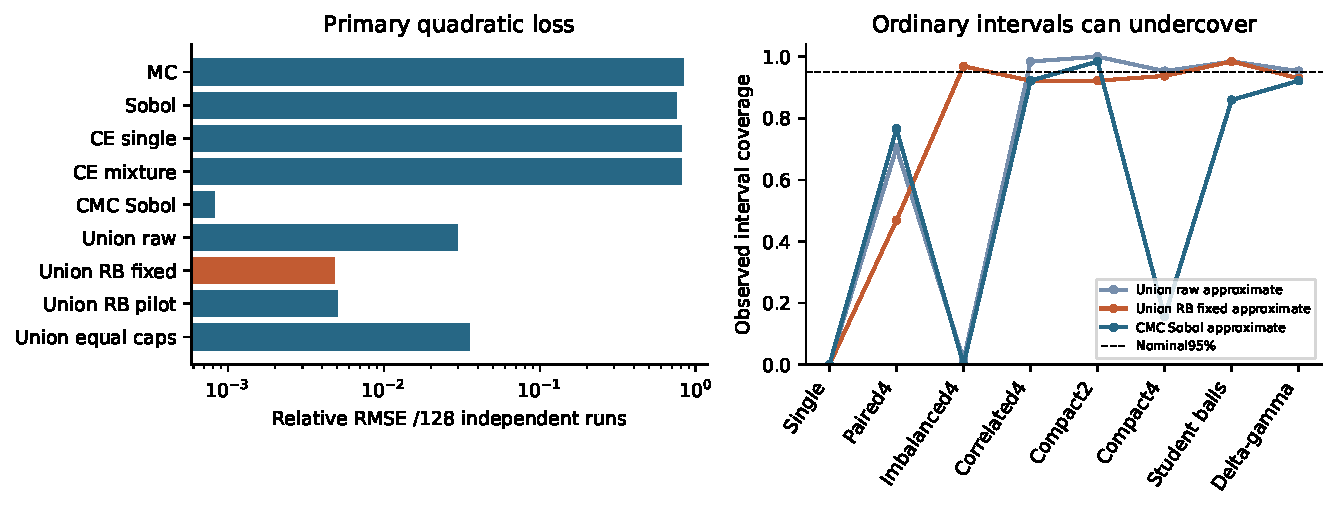
\includegraphics[width=\linewidth]{figures/primary_coverage.pdf}
\caption{Left: primary RRMSE across comparators. Right: ordinary approximate interval coverage varies sharply across workloads. The bounded probability intervals are a separate procedure; a tiny reported standard error can coexist with undercoverage.}
\end{figure}
\begin{table}[t]
\centering\small
\caption{Secondary and primary RRMSE at 16,384 calls. These three methods share analytic model access, though their sampling distributions differ. Every predefined case is included.}
\begin{tabular}{lrrr}\toprule
Problem & Union raw & Union fixed projection & Conditional Sobol\\\midrule
Single normal & 4.337e-16 & 4.337e-16 & 4.337e-16 \\
Paired4 & 3.401e-05 & 2.321e-05 & 0.677 \\
Imbalanced4 & 3.785e-06 & 1.672e-08 & 0.05444 \\
Correlated4 & 0.001978 & 0.001483 & 0.006837 \\
Compact2 & 0.008464 & 0.008147 & 1.275e-05 \\
Compact4 & 0.029 & 0.01849 & 0.9213 \\
Student balls & 0.04353 & 0.02737 & 0.2179 \\
Delta--gamma & 0.0297 & 0.004839 & 0.000821 \\
\\[-7pt]\bottomrule
\end{tabular}
\end{table}
The compact two-dimensional problem is a decisive counterexample to a broad advantage claim: conditional Sobol's RRMSE is approximately $1.27\times 10^{-5}$, versus $8.15\times 10^{-3}$ for fixed projected union sampling. Conversely, known affine unions make raw ALOE extremely accurate, leaving little useful work for adaptation. These cases demonstrate why an event definition aligned with a proposal can manufacture an impressive comparison if alternatives are omitted.

\begin{figure}[t]
\centering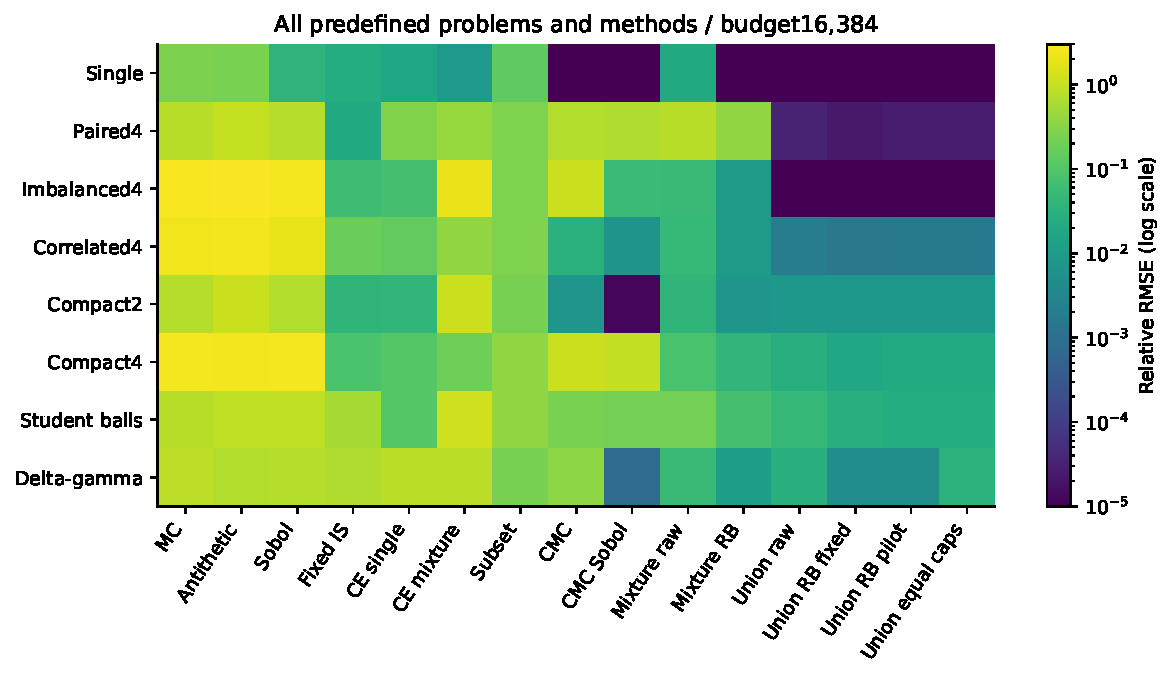
\includegraphics[width=\linewidth]{figures/suite.pdf}
\caption{Full predefined suite at 16,384 calls. Color encodes RRMSE on a logarithmic scale, clipped for display at $10^{-5}$ and 3. Machine-exact one-dimensional cases can be smaller; raw JSON preserves all values. Fifteen established baselines and implementation variants are shown without selective omission.}
\end{figure}

\subsection{The omitted-mode counterexample}
Let $ A=\{|Z|>b\}$ with $\bar\Phi(b)=5\times 10^{-6}$, and sample from
\begin{equation}
 q=0.9\,p(\cdot\mid Z>b)+0.1p.
\end{equation}
The likelihood-corrected estimator is unbiased and has full support. The hidden negative tail has proposal mass $5\times 10^{-7}$, so 20,000 samples miss it with probability $(1-5\times 10^{-7})^{20000}=0.9900498 $. Across 512 prescribed runs, the hidden mode was missed 99.414\% of the time. Median observed tail ESS was 17,999.5. Normal-interval coverage was only $3/512=0.586\%$; bounded Bernstein coverage was 512/512, with appropriately wide intervals. This is an explicit reliability failure, not a novel impossibility theorem.

\begin{figure}[t]
\centering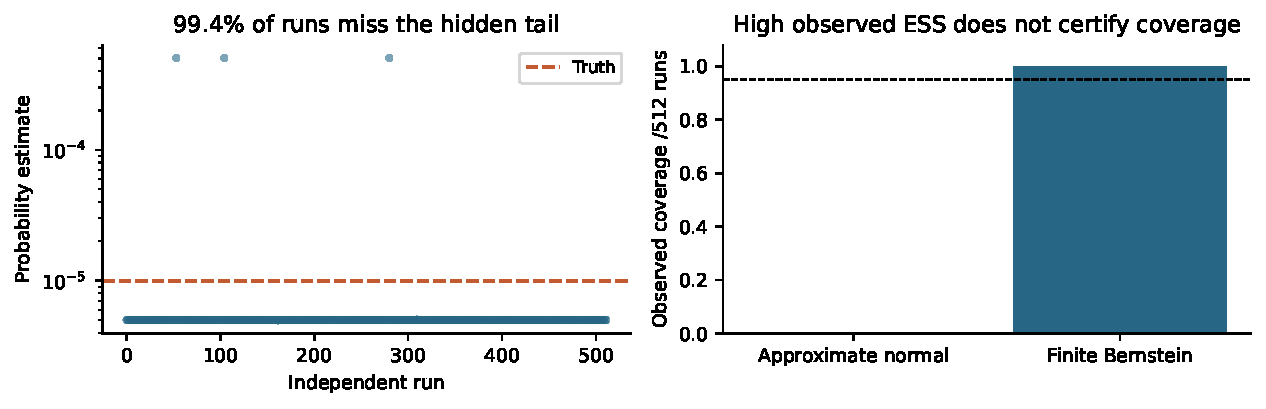
\includegraphics[width=\linewidth]{figures/missed_mode.pdf}
\caption{The complete 512-run omitted-mode experiment. Most estimates lie near half the true probability; rare large contributions preserve expectation. Ordinary intervals fail despite large observed ESS. Finite bounds retain coverage by refusing an unsupported narrow conclusion.}
\end{figure}
For a frozen uncovered region with zero hits in $ m $ independent nominal audit draws, its exact one-sided $1-\delta $ upper mass bound is $1-\delta^{1/m}$. At $ m=65,536 $, $\delta=.05 $, this is $4.5710\times 10^{-5}$, larger than the full target probability. Certifying residual mass at most $10^{-6}$ with audit error $.025 $ needs 3,688,878 zero-hit nominal draws. The structural cover avoids that generic audit by using a proved property of the supported model. It does not solve cheap discovery for arbitrary unknown loss functions.

\subsection{Modern adaptive comparison scope}
A separate paper-informed SAIS reproduction implements full-covariance proposals, local reassignment, subset thresholds, deterministic-mixture weights, tempering, covariance shrinkage and recycling. The source-to-equation concordance documents ambiguities and every disambiguation. Its independent-confirmation extension is separated from its paper-style recycled diagnostic, whose finite-sample properties are not silently inherited.

At the paper's stated linear-example settings ($ N=5 $, $ K=3000 $),24 independent runs gave recycled RRMSE 2.58\%; the separate confirmation extension gave 0.60\% with ordinary coverage 23/24. Smaller pilot budgets failed materially on other examples. These are exploratory tests, not reproduction of a published result table and not an equal-budget primary comparison. FAMIS remains unbenchmarked. No state-of-the-art dominance claim follows.

\section{VaR, severity and financial-model uncertainty}
Using a fixed proposal at a prespecified lowest threshold yields a monotone estimated survival curve. We invert it for VaR and use\eqref{eq:es} for ES. The finite-grid VaR bracket uses simultaneous Bonferroni probability bounds at all declared grid points. It is distinct from a pointwise interval at a data-chosen quantile. All such estimates are finite-sample biased plug-ins.

A separate 32-replication accuracy check uses normal-max and delta-gamma truth at 99\% and 99.9\%, budget 8192. The grid is \emph{oracle-centered}, using independent true VaR $\pm 0.35 $ to isolate numerical estimation; this does not validate automatic grid discovery. VaR RMSE ranged 0.00452--0.00525 risk units, and ES RMSE 0.00476--0.00718. Finite grid brackets covered all reference quantiles, but ordinary VaR coverage ranged 81.25--93.75\% and ES coverage 90.625--93.75\%. Thirty-two runs give substantial coverage uncertainty. These diagnostics do not support a blanket nominal 95\% VaR/ES inference claim.

Probability contribution bounds do not bound unbounded severity. Positive quadratic Student losses require $\nu>2 $ for a finite tail mean and generally $\nu>4 $ for conventional second-moment standard errors. The API rejects unsupported mean claims and omits unsupported severity standard errors. Bounded-above compact losses are treated separately. The implemented moment checks are sufficient conservative conditions, not complete symbolic moment classification.

\subsection{A separate chronological FX check}
Public Federal Reserve H.10 data provide USD values of EUR, JPY and GBP \citep{fedh10}. Original source HTML, retrieval receipts and SHA-256 hashes are retained. JPY quotes are inverted; complete-case dates are aligned before returns with no forward filling. The equal-dollar basket loss is minus the mean simple currency return. Consecutive observations can span weekends or holidays; no carry, interest or transaction costs are modeled. The saved revised data vintage is not a point-in-time vintage.

Both prespecified unconditional families are fitted only on 2000--2014 (3769 returns), then frozen for 2015--2025 (2748 returns). The Student maximum-likelihood fit has $\nu=6.4280 $. At 99\%, Gaussian VaR/ES are 1.0883\%/1.2470\%; Student VaR/ES are 1.1949\%/1.5186\%. Thus model choice changes ES by 21.8\%, far more than a small simulation error bar would imply. Evaluation exceedances are 32 and 18, versus 27.48 expected under exact 1\% calibration. Neither count alone validates a distribution.

We retain all 16,488 forecast/residual records. Diagnostics include exceedance residuals, $ e-q-(L-q)_+/\beta $, and the joint FZ0 score \citep{patton2019}, with 20-observation circular block bootstrap and 1000 paired resamples. At 95\%, both families have too few exceedances (95 Gaussian and 105 Student versus 137.4 expected); their block-bootstrap VaR calibration intervals exclude zero. Student scores improve at 95\%, while 97.5\% and 99\% comparisons are unresolved; Gaussian 99\% ES residual uncertainty is borderline. A fixed 20-observation block rule is an assumption, not a universal dependence correction. These checks concern observable historical calibration. They cannot empirically verify daily probabilities of $10^{-5}$, establish the joint dependence model used by the synthetic engine, or show regulatory compliance. Basel's use of stressed ES motivates the severity question, not a compliance claim \citep{basel}.

\section{Implementation, adversarial review and reproducibility}
The software exposes callable model, probability, attribution, VaR/ES and baseline APIs. A local-only black/green investigation interface shows actual computed results, the finite interval, separate diagnostic errors, weighted branch contributions and exported seed/configuration records. Branch attribution integrates the argmax partition; it is neither causal attribution nor the proportion of proposal draws allocated to a branch. Prefix traces are recorded sample means and do not create optional-stopping guarantees.

Independent agents reviewed raw code and artifacts, including an adversarial reviewer instructed to disprove the improvement. They found overly permissive symmetry checks, scaled-discriminant failures, support underflow, Student moment issues, a clipped-interval display mismatch and severity cancellation. The corresponding regression tests and original evidence are retained. This is agent-based independent review, not external human peer review. The failed primary comparison remains unchanged by rhetorical interpretation.

The source tree includes mathematical assumptions, exact random seeds, original protocols, support amendments, immutable executed source snapshots, raw runs, aggregation hashes, figure-generation code, historical source receipts and a SAIS fidelity record. Scripts refuse to overwrite completed experiment directories. Verification checks hashes rather than trusting README claims. Initial experiments used Python 3.14.7, NumPy 2.5.4 and SciPy 1.18.1 on ARM 64 macOS CPU. No CUDA or energy result is reported. Hardware memory telemetry was denied; process RSS is explicitly limited.

\section{Limitations and research verdict}
The strongest useful result is a bounded, inspectable estimator for a supported structural loss family, together with robust negative evidence. It cannot estimate arbitrary black-box losses using the same analytic oracle; it cannot certify an unknown market distribution; and it did not beat the strongest tested simple method on the primary cost criterion. ALOE, conditional Monte Carlo and concentration bounds explain its mathematical properties. The particular engineering composition has not survived a proof of global novelty.

A defensible future research contribution would require an identifiable new cover construction, a sharper conditional-allocation theorem, or a generic discovery guarantee with explicit assumptions, followed by fair comparison against modern learned proposals. Adding more mixture components, neural networks or a more elaborate interface would not resolve the failed hypothesis. The present artifact supports correctness within stated limits and a reproducible performance comparison. The original-estimator breakthrough remains unachieved.

\appendix
\section{Independent reference formulas}
For independent Gaussian maxima with offsets $ d_i $,
\begin{equation}
 \Pp(\max_i(Z_i+d_i)>t)=1-\prod_i\Phi(t-d_i).
\end{equation}
The implementation evaluates the log product and uses \texttt{expm1} to avoid rare-tail cancellation. For disjoint balls $ A_j=\{\|Z-m_j\|^2<r_j^2-t\}$,
\begin{equation}
 \Pp(L>t)=\sum_jF_{\chi'^2_d(\|m_j\|^2)}((r_j^2-t)_+),\qquad t\ge 0.
\end{equation}
Overlapping interiors are rejected by the additive reference. For Student factors, condition on $ S=s $ and replace radius and noncentrality arguments by $(r_j^2-t)s/\nu $ and $\|m_j\|^2s/\nu $, then integrate the chi-square scale. These calculations are independent of the line-root estimator. Special-function and adaptive-quadrature error diagnostics are not rigorous numerical enclosures.

\section{Cost and estimator assumptions at a glance}
\begin{itemize}
\item A fixed pilot may choose cover/proposal/direction. Confirmation must be independent; adaptive reuse requires a different proof.
\item Union sampling needs exact halfspace masses and conditional samplers. It uses explicit target density structure; a sampling-only target is insufficient for the same formulas.
\item All failure intervals and maximum-branch crossings matter. A single positive root is invalid for nonmonotone losses.
\item Bounds certify sampling error under the assumed model and exact-arithmetic idealization. Float 64 tests establish numerical evidence within the exercised range.
\item Common seeds are reproducibility labels; they do not make different algorithm samples identical or automatically justify paired inference.
\item Accuracy-per-cost results include unsuccessful training and preparation. Equal nominal budgets do not imply equal used evaluations or equal information.
\item Historical model checks and extreme synthetic probability checks answer different questions; neither substitutes for the other.
\end{itemize}

\raggedright
\bibliographystyle{plainnat}
\bibliography{references}
\end{document}
